\documentclass[a4paper]{article}

%% Language and font encodings
\usepackage[english]{babel} \usepackage[utf8x]{inputenc}
\usepackage[T1]{fontenc}

%% Sets page size and margins
\usepackage[a4paper,top=3cm,bottom=2cm,left=3cm,right=3cm,marginparwidth=1.75cm]{geometry}

%% Useful packages
\usepackage{amsmath} 
\usepackage{amsfonts}
\usepackage{mathtools} 
\usepackage{graphicx}
\usepackage{bm} % bold math
\usepackage[colorinlistoftodos, textsize=footnotesize]{todonotes}
\usepackage[colorlinks=true, allcolors=blue]{hyperref}
\usepackage{setspace}
\usepackage{algorithm2e}
\usepackage{hyperref}

%% For listing source code.
\usepackage{listings}
\usepackage{xcolor} % for setting colors

\definecolor{mygreen}{RGB}{26, 148, 49}

% set the default code style
\lstset{
    frame=tb, % draw a frame at the top and bottom of the code block
    tabsize=4, % tab space width
    showstringspaces=false, % don't mark spaces in strings
    numbers=left, % display line numbers on the left
    commentstyle=\color{mygreen}, % comment color
    keywordstyle=\color{blue}, % keyword color
    stringstyle=\color{red} % string color
}

\newif\ifcompile
%\compiletrue % uncomment out to compile

\newtheorem{remark}{Remark}

\DeclareMathOperator*{\argmin}{arg\,min}

\newcommand{\bgamma}{{\bm\gamma}}
\newcommand{\btgamma}{{\bm{\tilde\gamma}}}
\newcommand{\vv}[1]{{\bm{#1}}}

\newcommand{\smalltodo}[2][]
{\todo[caption={#2}, #1]
	{\begin{spacing}{0.5}#2\end{spacing}}}

\newcommand{\AlejandroComment}[2][]{\smalltodo[color=purple!40,
author=Alejandro, #1]{#2}{}}
	
\newcommand{\ShermComment}[2][]{\smalltodo[color=blue!40, author=Sherm,
#1]{#2}{}}
	
\newcommand{\XuchenComment}[2][]{\smalltodo[color=green!40, author=Xuchen,
		#1]{#2}{}}
	
\newcommand{\SeanComment}[2][]{\smalltodo[color=cyan!40, author=Sean, #1]{#2}{}}
	
\newcommand{\DamrongComment}[2][]{\smalltodo[color=magenta!40, author=Damrong,
		#1]{#2}{}}

\title{SoftSim Geometric Query Specifications} 

\author{Alejandro M. Castro}

\begin{document}
\maketitle

%\begin{abstract}
%Your abstract.
%\end{abstract}

\section{Introduction}

The purpose of this document is to describe a practical geometry query to be
\AlejandroComment{A comment with my name and fav color}
used in the simulation of soft bodies with contact. There is a large variety of
mathematical formulations with strong foundations in the FEM community. While
the Mortar method seems to be a standard in the FEM community
\cite{bib:yang2005, bib:delorenzis2014, bib:fischer2006, bib:popp2010} here
we'll follow an approach based on the work by Duriez
\cite{bib:duriez2006_realistic_haptic_rendering} given it's simplicity and the
accuracy requirements for the short-term applications. Further research on
Mortar methods and its variants must be conducted but we believe this to be a
good starting point, especially regarding the practical definition of a contact query.

\subsection{Geometry Outline}
A brief description of the query requirements are given in 
\cite[\S 3.2]{bib:duriez2006_realistic_haptic_rendering}.

In a nutshell, given two surface meshes $A$ and $B$, the geometric query identifies a set of
$n_c$ point contact pairs. For each pair, the query reports points $Ca$ and $Cb$
on surfaces $A$ and $B$ respectively, the contact normals $\widehat{n}_A$ and
$\widehat{n}_B$ at these points on each surface and the barycentric coordinates
of $Ca$ and $Cb$ within the triangle the belong to. The physics solver is agnostic to
how these pairs are obtained and, hopefully, robust to geometry induced
perturbations such as changes in the normal directions especially at sharp
corners.

Figure \ref{fig:pq_definition} (Fig. 2 in
\cite{bib:duriez2006_realistic_haptic_rendering}) shows an example of two points
$P$ and $Q$ identified by the query. While point $Q$ in the figure corresponds
to a surface vertex, point $P$ is described by the barycentric coordinates in
the triangle it belongs to.

\begin{figure}[!h]
	\centering
	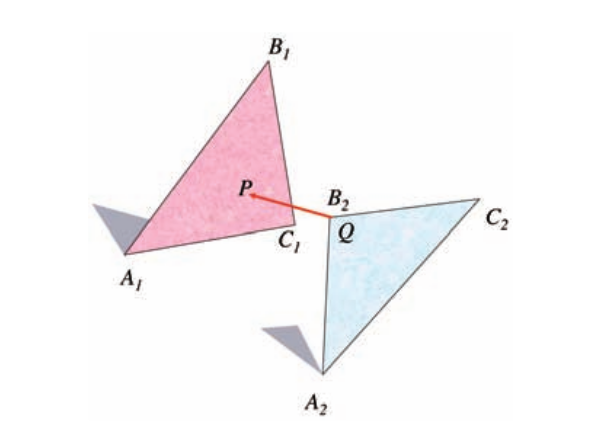
\includegraphics[width=0.5\columnwidth]{figures/PQdefinition.png}
	\caption{\label{fig:pq_definition} 
	An example of two points $P$ and $Q$ identified by the query.}
\end{figure}

In \cite{bib:duriez2006_realistic_haptic_rendering} other contact modes are
identified, summarized in Fig. \ref{fig:contact_modes} (Fig. 3 in
\cite{bib:duriez2006_realistic_haptic_rendering}). The two top figures
correspond to the most probable cases given that for the cases outlined in the
bottom row triangles must be in perfect alignment. Even if those cases are
considered, the information consumed by the physics engine is the same.

\begin{figure}[!h]
	\centering
	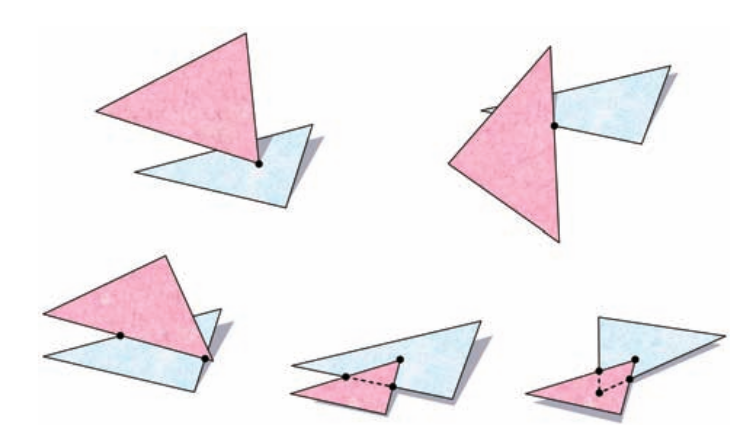
\includegraphics[width=0.5\columnwidth]{figures/different_cases.png}
	\caption{\label{fig:contact_modes} 
	Different contact scenarios for triangle-triangle pairs.}
\end{figure}

\subsection{Geometry Specification by the Physics Engine}

The FEM model for soft bodies is discretized using meshes of tetrahedra. The
geometry used for contact queres does not necessarily need to be represented by
the same mesh used for FEM, and actually in \cite{bib:duriez2013thesis} usually
a coarser mesh is used for contact queries. Whether this is true for us or not,
the geometry engine does not need to know this details and the FEM solver could
opt for using different representations with the additional bookkeeping. 

It is very important that there is a precise correspondence
between the mesh used by the physics engine and the mesh used by the geometry
engine. That is, indexes reported back by the geometry engine must make sense to
the physics engine. This leads to the conclusion: 
\begin{itemize}
	\item The physics engine must be able to specify the mesh in its entirety,
	including vertex positions and connectivity.
\end{itemize}

This is different from the typical approach for rigid contact, in which the
physics engine does not know about the actual geometric representation.

Given the FEM solver knows and understands the structure of the geometry, it can
already provide to the geometry engine:
\begin{enumerate}
	\item Vertex positions in a \textit{reference configuration} (typically
	the zero stresses state) and connectivity.
	\item Surface vertex normals. Within each triangular face normals are
	linearly interpolated given their barycentric location when needed.
\end{enumerate}

\subsection{Geometric Queries}
\label{sec:geometric_queries}

In this section we provide a more detailed description of the query. It is a
``constructive'' description in that we provide a methodology to compute it. The
reason we need a constructive description is because the queries are usually
performed at \textit{unphysical states} at which interpenetration already
ocurred. In the real world, contact leads to surfaces that deform conforming to
each other, even if only in a microscopic region. Therefore, given two objects,
the real physics leads to surfaces that conform and are \textit{parallel} to
each other. In that state, two closest neighbor points on each body have
coincident locations and the normals on each body are exactly opposite to each
other. This is generally not true in the discrete setting, however just an
approximation to the real physics. Therefore in what follow we'll be specific to
this constructive approach, with remarks to the physical approximation when it
corresponds. 

Consider two bodies $A$ and $B$, each with their surface discretized by a
triangle mesh. We will first find the set of surface vertices $C_a$ of $A$ that
lie inside of $B$. We'll denote that set with ${}^A\mathcal{C}$. For each
surface vertex $C_a$ of $A$ inside $B$ the contact query must find a point $C_b$
on the surface of $B$ that is \textit{close} to $C_a$. Even if $C_b$ is the
closest point to $C_a$ on $B$, usually the surface normals evaluated at $C_a$
and $C_b$ will not be the opposite of each other. This is a consequence of the
queries performed at \textit{unphysical states} as outlined in the previous
paragraph. However, these states are usually a good approximation in the limit
in which the surfaces conform to each other. Now, this fact leads to a choice;
``in what direction do we search $C_b$ on $B$ from $C_a$?'' we could search for
the \textit{closest point}, i.e. the direction is aligned with the normal on
$B$, or we could search in the direction to the normal to $A$. Other options are
possible, but it is important to keep in mind that the normals on $A$ and $B$ do
align in the limit in which the discrete solution converges as the spatial
resolution increases. From a practical standpoint however, we do know the
normal vector $\widehat{n}_A$ at $C_a$ on $A$'s surface. Therefore it makes
sense to use $\widehat{n}_A$ as the search direction from $C_a$ onto $B$'s
surface to find $C_b$. This approach has the nice effect of uniquely defining
the result of the query.

Similarly, we define the set ${}^B\mathcal{C}$ by finding for each surface vertex
$C_b$ of $B$, a corresponding point $C_a$ on surface $A$ by essentially
ray casting from $C_b$, in the direction of $\widehat{n}_B$ at $C_b$ (since it's
known), onto the surface of $A$. The set of all collision pairs will be
denoted with $\mathcal{C} = {}^A\mathcal{C} \bigcup
{}^B\mathcal{C}$.
 
For each of these pairs $C_a$/$C_B$ the query must provide:
\begin{itemize}
\item Contact pair $C_a$, $C_b$.
\item Indices of the surface triangles to which points $C_a$ and $C_b$ belong,
in their respective surfaces.
\item Barycentric coordinates of $C_a$ and $C_b$ in their triangles.
\item Surface normals $\widehat{n}_A$ and $\widehat{n}_B$. This can be evalated
by interpolation given we know in advance the surface vertex normals and the
barycentric coordinates are a result of this query.
\end{itemize}

This information can be reported as point pairs by embeding this information in
a data structure outlined in Listing \ref{lst:data_struct}. Notice that in this
format, the physics engine is agnostic to the specifics of the query.

\begin{lstlisting}[language=C++, caption={Contact feature data structure}\label{lst:data_struct}]
	template <typename T>
	struct MeshMeshContactFeature {
		// Feature specs on mesh A.
		GeometryId id_A;           // Geometry identifier for mesh A.     
		Vector3<T> p_WCa;          // Position of point Ca on A's surface.
		SurfaceFaceIndex Ca_face;  // A face to which Ca belongs.
		SurfaceMesh<T>::Barycentric
			Ca_barycentric;        //  Barycentric coordinates of
								   //  point Ca in triangle Ca_face.
		Vector3<T> normal_Ca_W;    //  Outward normal at Ca, expressed in W.						   
	
		// Feature specs on mesh B.
		GeometryId id_B;           // Geometry identifier for mesh B.
		Vector3<T> p_WCb;          // Position of point Cb on B's surface.
		SurfaceFaceIndex Cb_face;  // A face to which Cb belongs.
		SurfaceMesh<T>::Barycentric
			Cb_barycentric;        //  Barycentric coordinates of
								   //  point Cb in triangle Cb_face.
		Vector3<T> normal_Cb_W;    //  Outward normal at Cb, expressed in W.								   
	};		
\end{lstlisting}

\subsubsection{Edge to Edge contact. Andy maybe other special cases?}
The formulation to be presented in what follows can deal with edge-edge
collisions within the same framework if we just only augment
$\mathcal{C}$ to also include edge-edge point pairs, providing exactly
the same information described above. This corresponds to the top-right corner
in Fig. \ref{fig:contact_modes}.

That is, if there is an edge-edge intersection, the collision engine should be
able to provide point $C_b$ on a given edge of $B$ and point $C_a$ on a given
edge of $A$ that are the closest within those edges. Once again, if we
encapsulate this information as points that belong to given triangles, these
triangles' indexes and the barycentric coordinates contain all the information
we need.



\bibliographystyle{ieeetr} \bibliography{geometry_query_specs}

\listoftodos

\end{document}
